%%%%%%%%%%%%%%%%%%%%%%%%%%%%%%%%%%%%%
%                                   %
% Compile with XeLaTeX and biber    %
%                                   %
% Questions or comments:            %
%                                   %
% joshua dot mcneill at uga dot edu %
%                                   %
%%%%%%%%%%%%%%%%%%%%%%%%%%%%%%%%%%%%%

\documentclass{beamer}
  % Read in standard preamble (cosmetic stuff)
  %%%%%%%%%%%%%%%%%%%%%%%%%%%%%%%%%%%%%%%%%%%%%%%%%%%%%%%%%%%%%%%%
% This is a standard preamble used in for all slide documents. %
% It basically contains cosmetic settings.                     %
%                                                              %
% Joshua McNeill                                               %
% joshua dot mcneill at uga dot edu                            %
%%%%%%%%%%%%%%%%%%%%%%%%%%%%%%%%%%%%%%%%%%%%%%%%%%%%%%%%%%%%%%%%

% Beamer settings
% \usetheme{Berkeley}
\usetheme{CambridgeUS}
% \usecolortheme{dove}
% \usecolortheme{rose}
\usecolortheme{seagull}
\usefonttheme{professionalfonts}
\usefonttheme{serif}
\setbeamertemplate{bibliography item}{}

% Packages and settings
\usepackage{fontspec}
  \setmainfont{Charis SIL}
\usepackage{hyperref}
  \hypersetup{colorlinks=true,
              allcolors=blue}
\usepackage{graphicx}
  \graphicspath{{../../figures/}}
\usepackage[normalem]{ulem}
\usepackage{enumerate}

% Document information
\author{M. McNeill}
\title[FREN2001]{Français 2001}
\institute{\url{joshua.mcneill@uga.edu}}
\date{}

%% Custom commands
% Lexical items
\newcommand{\lexi}[1]{\textit{#1}}
% Gloss
\newcommand{\gloss}[1]{`#1'}
\newcommand{\tinygloss}[1]{{\tiny`#1'}}
% Orthographic representations
\newcommand{\orth}[1]{$\langle$#1$\rangle$}
% Utterances (pragmatics)
\newcommand{\uttr}[1]{`#1'}
% Sentences (pragmatics)
\newcommand{\sent}[1]{\textit{#1}}
% Base dir for definitions
\newcommand{\defs}{../definitions}


  % Packages and settings
  \usepackage{phonrule}
  % This is the preamble package and settings for drawing a flowchart of how
% to do phonological analysis
\usepackage{tikz}
  \usetikzlibrary{shapes.geometric, arrows, positioning}
  \tikzstyle{process} = [rectangle,
                         text centered,
                         draw=black,
                         align=center]
  \tikzstyle{arrow} = [thick,->]

  \usepackage[backend=biber, style=apa]{biblatex}
    \addbibresource{../references/References.bib}

  % Document information
  \subtitle[Phonological Analysis]{Phonological Analysis of Data}

  %% Custom commands
  % Subsection/frame titles
  \newcommand{\suboneone}{When we have more data}
  \newcommand{\subonetwo}{The general process}
  \newcommand{\subonethree}{Be careful}
  \newcommand{\subonefour}{Practice}

\begin{document}
  % Read in the standard intro slides (title page and table of contents)
  %%%%%%%%%%%%%%%%%%%%%%%%%%%%%%%%%%%%%%%%%%%%%%%%%%%%%%%%%%%%%%%%
% This is a standard set of intro slides used in for all slide %
% documents. It basically contains the title page and table of %
% contents.                                                    %
%                                                              %
% Joshua McNeill                                               %
% joshua dot mcneill at uga dot edu                            %
%%%%%%%%%%%%%%%%%%%%%%%%%%%%%%%%%%%%%%%%%%%%%%%%%%%%%%%%%%%%%%%%

\begin{frame}
  \titlepage
  \tiny{Office: % Basically a variable for office hours location
Gilbert 121\\
        Office hours: % Basically a variable for office hours
 lundi, mercredi, vendredi 10:10--11:10
}
\end{frame}

\begin{frame}
  \tableofcontents[hideallsubsections]
\end{frame}

\AtBeginSection[]{
  \begin{frame}
    \tableofcontents[currentsection,
                     hideallsubsections]
  \end{frame}
}


  \section{Phonological Analysis}
    \subsection{\suboneone}
      \begin{frame}[t]{\suboneone}
          \begin{block}{An English example}
            \only<1-2>{
              Are [ɹ] and [ɹ̥] phonemes or allophones?
            }
            \only<3->{
              What are the phonological rules at play?
            }
          \end{block}
          \only<1-2>{
            \begin{block}{The data}
              \begin{tabular}{r l | r l}
                \lexi{pray}   & [ˈpʰɹ̥eɪ]   & \lexi{gray}    & [ˈɡɹeɪ] \\
                \lexi{crab}   & [ˈkʰɹ̥æb]   & \lexi{par}     & [ˈpʰɑɹ] \\
                \lexi{broker} & [ˈbɹoʊ.kɹ̩] & \lexi{fresh}   & [ˈfɹ̥ɛʃ] \\
                \lexi{regain} & [ɹiˈɡeɪn]  & \lexi{shriek}  & [ˈʃɹ̥ik] \\
                \lexi{tar}    & [ˈtʰɑɹ]    &                &
              \end{tabular}
            \end{block}
            \begin{block}<2->{}
              Are there any minimal pairs?
            \end{block}
          }
          \only<3-6>{
            \begin{columns}
              \column{0.45\textwidth}
                \begin{block}{The data}
                  \begin{tabular}{r @{\_\_} l | r @{\_\_} l}
                    \multicolumn{2}{c}{[ɹ̥]} & \multicolumn{2}{c}{[ɹ]} \\
                    \hline
                    {[}ˈpʰ  & eɪ]           & [ˈɡ   & eɪ] \\
                    {[}ˈkʰ  & æb]           & [\#   & iˈɡeɪn] \\
                    {[}ˈf   & ɛʃ]           & [ˈtʰɑ & \#] \\
                    {[}ˈʃ   & ik]           & [ˈpʰɑ & \#] \\
                            &               & [ˈb   & oʊ.kɹ̩]
                  \end{tabular}
                \end{block}
              \column{0.51\textwidth}
                \begin{block}{\only<3-4>{What are the environments as natural classes?}\only<5->{\alert{Are there complementary environments?}}}
                  \begin{itemize}
                    \item<4-> {[}ɹ̥] \alert<6->{after voiceless obstruents}, before vowels
                    \item<4-> {[}ɹ] \alert<6->{after voiced obstruents} and vowels, before vowels, word-initial, word-final
                  \end{itemize}
                \end{block}
            \end{columns}
          }
          \only<7-8>{
            \begin{block}{Which allophone is also the phoneme?}
              \uncover<8->{
                It's the one that occurs in more environments: [ɹ]
              }
            \end{block}
            \begin{block}<8->{Two types of allophones}
              \begin{itemize}
                \item \alert{Basic allophones}: % Basic allophone
An allophone that appears in many different environments

                \item \alert{Restricted allophones}: % Restricted allophone
An allophone that appears in only a small number of environments

              \end{itemize}
            \end{block}
          }
        \only<9->{
          \begin{block}{Finally}
            \begin{itemize}
              \item \phonl{/ɹ/}{[ɹ̥]}{\phonfeat{+voiceless \\ +obstruent}}
              \item \phonc{/ɹ/}{[ɹ]}{elsewhere}
            \end{itemize}
          \end{block}
        }
      \end{frame}

    \subsection{\subonetwo}
      \begin{frame}{\subonetwo}
        \small% This draws a flow chart for how to do phonological analysis
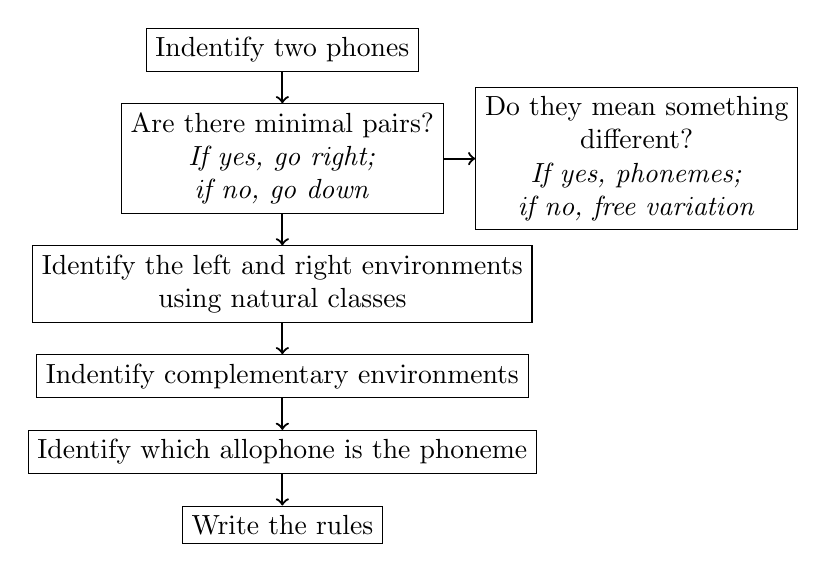
\begin{tikzpicture}
  \node (sounds)   [process]                          {Indentify two phones};
  \node (minpairs) [process, below=0.4cm of sounds]   {Are there minimal pairs?\\
                                                       \emph{If yes, go right;}\\
                                                       \emph{if no, go down}};
  \node (meaning)  [process, right=0.4cm of minpairs] {Do they mean something\\
                                                       different?\\
                                                       \emph{If yes, phonemes;}\\
                                                       \emph{if no, free variation}};
  \node (environs) [process, below=0.4cm of minpairs] {Identify the left and right environments\\
                                                       using natural classes};
  \node (compenvs) [process, below=0.4cm of environs] {Indentify complementary environments};
  \node (phoneme)  [process, below=0.4cm of compenvs] {Identify which allophone is the phoneme};
  \node (rule)     [process, below=0.4cm of phoneme]  {Write the rules};
  \draw [arrow] (sounds)   -- (minpairs);
  \draw [arrow] (minpairs) -- (meaning);
  \draw [arrow] (minpairs) -- (environs);
  \draw [arrow] (environs) -- (compenvs);
  \draw [arrow] (compenvs) -- (phoneme);
  \draw [arrow] (phoneme)  -- (rule);
\end{tikzpicture}

      \end{frame}

    \subsection{\subonethree}
      \begin{frame}{\subonethree}
        \only<1>{
          \begin{block}{No minimal pairs $\neq$ allophones}
            You must find the sounds in complementary distribution
          \end{block}
          \begin{example}
            No minimal pairs for [b] and [ɡ] in the data but they're in overlapping distribution:
            \begin{itemize}
              \item {[}ˈbɹoʊ.kɹ̩]
              \item {[}ˈɡɹeɪ]
            \end{itemize}
          \end{example}
        }
        \only<2>{
          \begin{block}{Rhyming doesn't matter}
            Minimal pairs can rhyme but don't have to
          \end{block}
          \begin{example}
            \begin{itemize}
              \item {[}ˈboʊt] and [ˈbɪt]: don't rhyme, are a minimal pair
              \item {[}ˈlɪ.ɾɹ̩] and [ˈɡlɪ.ɾɹ̩]: do rhyme, aren't a minimal pair
              \item {[}ˈdɔɡ] and [ˈlɔɡ]: do rhyme, are a minimal pair
            \end{itemize}
          \end{example}
        }
      \end{frame}

    \subsection{\subonefour}
      \begin{frame}{\subonefour}
        \begin{block}{Try these}
          \textcite{dawson_language_2016}, chapter 3 exercises 24, 25, 33, and 37
        \end{block}
      \end{frame}
\end{document}
